\shorttitle{Life Sciences}
\section{Life Sciences}

\begin{figure*}[ht]
  \begin{center}
   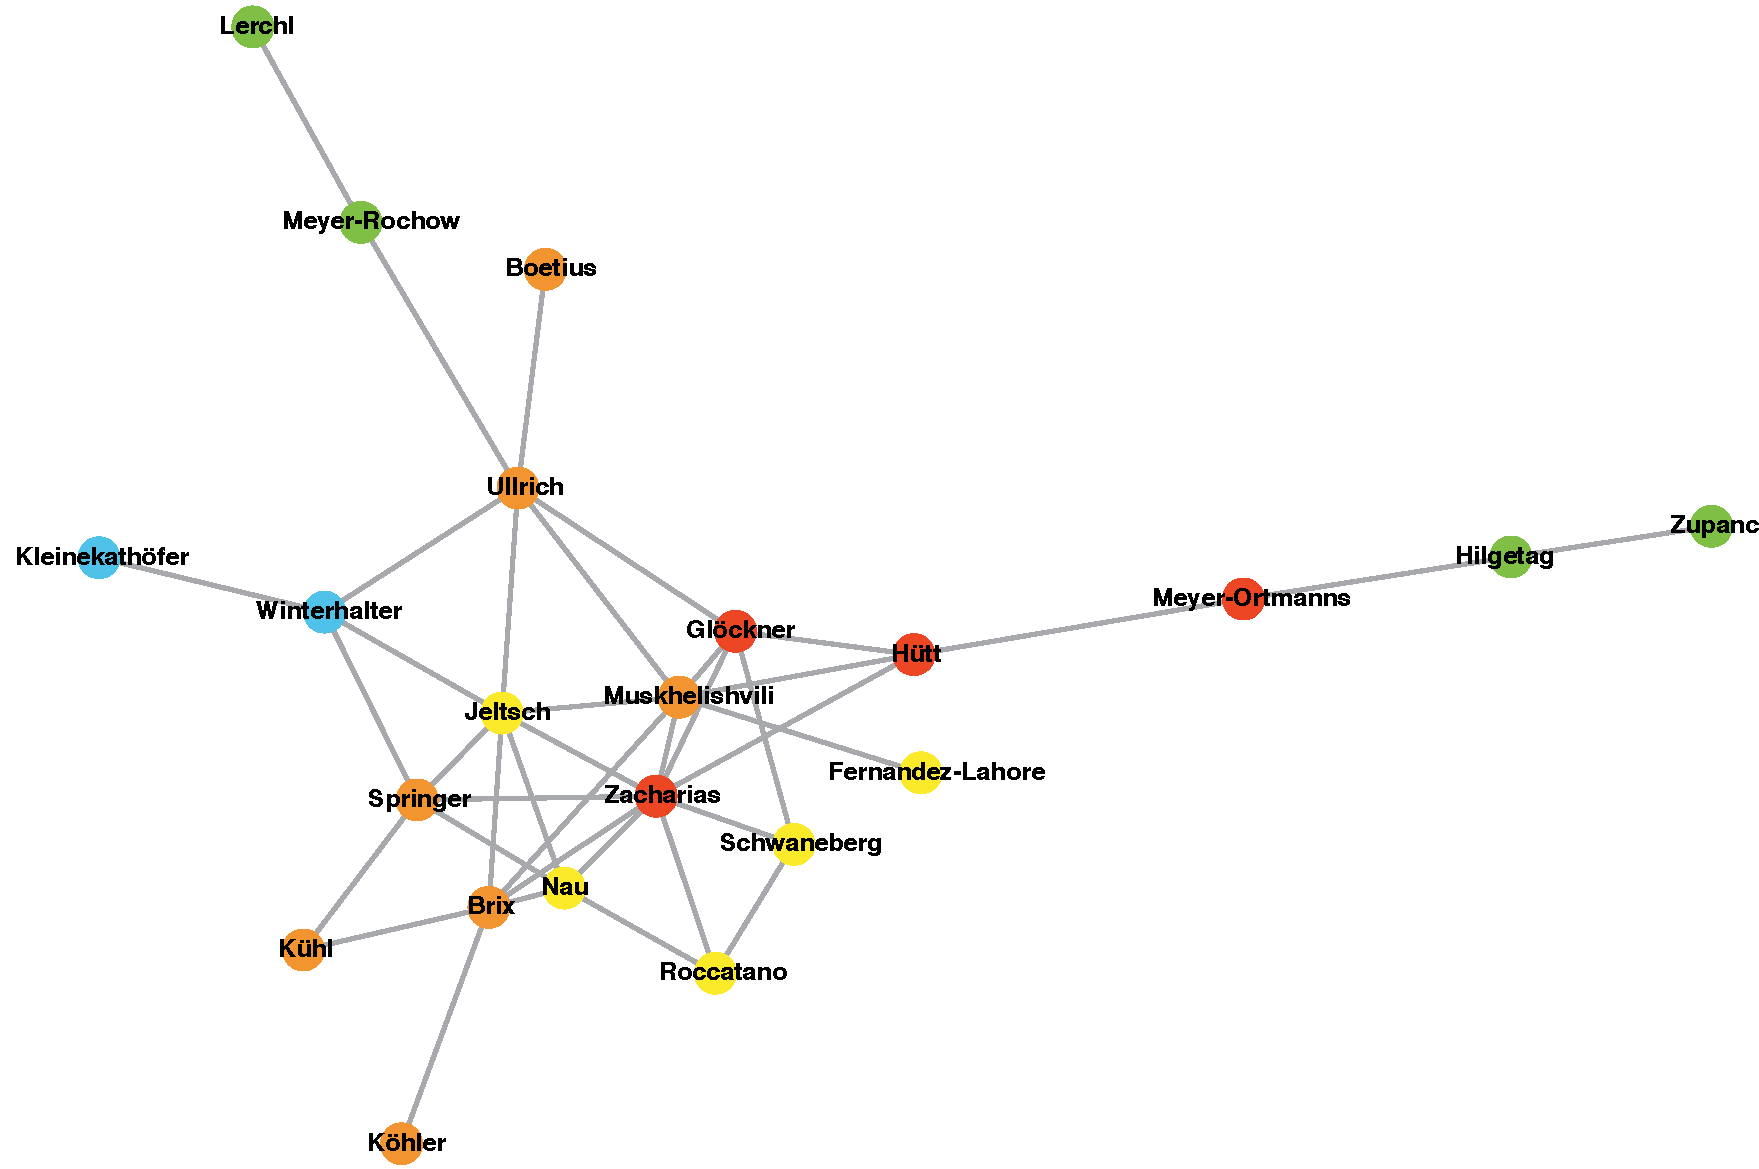
\includegraphics[width=\hsize]{network_LifeSci1_tmp03.pdf}
    \mycaption{Geometry and functionality of the complex biological network at Jacobs University Bremen that is formed by the interaction of Computational Biologists, Biophysicists, Biotechnologists, Neuroscientists, and Molecular Life Scientists.  }\label{fig:LifeSc}
   \end{center}
\end{figure*}


Life Scientists at IUB follow an integrated research approach that covers a variety of scientific fields and interests. The spectrum ranges from the analysis of molecules and their usage for biotechnological applications to the understanding of the mechanisms that explain the functions of complex systems like cells, organisms, and even entire habitat communities. Our research approaches combine experimental and theoretical work aiming towards future challenges in the target areas of the School of Engineering and Science. \\

The Life Scientists at IUB focus their research interests on
\begin{myitemize}
\item   the molecules and macromolecules which make up living matter,
\item the dynamical organization of genomes and cells,
\item   the biochemistry and physiology of life,
\item   the molecular mechanisms that maintain vital functions of cells, and
\item   the patho-physiological events which result in the onset of diseases.\\
\end{myitemize}


The research results provide us with insights into the molecular mechanisms that are found in microbes, plants and animals. Moreover, marine and terrestric habitats which are filled with life are analyzed in composition and interactivity. The perception of animals and human beings of their surrounding world is another important aspect of our research teams as is the modeling of complex systems like gene networks, metabolism, trafficking of molecules in cells, and interaction of living creatures in biological systems.\\

In 2006, a clear focus was on the spatial and temporal regulation of biological systems. Another important and recent advance is that the Molecular Life Scientists at IUB have filled their excellently designed and newly build research facilities and laboratories with life. Life Scientists at IUB have established numerous successful research collaborations within our research community. Above it, our research activities are embedded in the scientific communities of the Bremen-area and have attracted significant international attention. The nodes and edges that make up the units of the vital network of Life Scientists at IUB are illustrated in Figure \ref{fig:LifeSc}. \\




\textit{Perspectives}\\
The goal of the Life Scientists at IUB is to understand the function
of life, in its complexity and functional organization, on the
molecular and the systemic levels. We feel best prepared to further
evolve our research activities to face the major global challenges
of the future.
